\documentclass[tikz, border=5mm]{standalone}
\usepackage{tikz}
\usepackage[svgnames]{xcolor}
\usetikzlibrary{positioning, arrows.meta, calc}

\definecolor{myColor1}{HTML}{C0392B} % Pomegranate (a softer, deeper red)
\definecolor{myColor2}{HTML}{27AE60} % Nephritis (a pleasant, medium green)
\definecolor{myColor3}{HTML}{2980B9} % Belize Hole (a solid, medium blue)
\definecolor{myColor4}{HTML}{D35400} % Pumpkin (a warm, less sharp orange)
\definecolor{myColor5}{HTML}{8E44AD} % Wisteria (a softer purple)
\definecolor{myColor6}{HTML}{16A085} % Green Sea (a teal/cyan, darker than pure cyan)
\definecolor{myColor7}{HTML}{F39C12} % Orange (more of a dark yellow/light orange, less intense than pure yellow)
\definecolor{myColor8}{HTML}{C0399B} % A softer, slightly desaturated magenta/pink

% Helper commands for colored '1's (0s are black)
\newcommand{\B}[1]{{\color{black}#1}} % Black for 0s
\newcommand{\C}[2][1]{{\color{myColor#1}#2}} % \C[color_idx]{bit_value} - bit_value is always 1

% String definitions based on the derived coloring logic
% m (input): 0101010101010101 (8 ones, colors C1-C8)
\def\memstring{%
    \B0\C[1]{1}\B0\C[2]{1}\B0\C[3]{1}\B0\C[4]{1}\B0\C[5]{1}\B0\C[6]{1}\B0\C[7]{1}\B0\C[8]{1}%
}
% r1 = m
\def\rOnestring{\memstring}
% r1 >> 1 (7 ones, C1-C7, C8 is lost)
\def\rOneshiftedstring{%
    \B0\B0\C[1]{1}\B0\C[2]{1}\B0\C[3]{1}\B0\C[4]{1}\B0\C[5]{1}\B0\C[6]{1}\B0\C[7]{1}\B0%
}
% v1 = 0011111111111111 (14 ones, colors starting C2)
\def\vOnestring{\B0\C[1]{1}\C[1]{1}\C[2]{1}\C[2]{1}\C[3]{1}\C[3]{1}\C[4]{1}\C[4]{1}\C[5]{1}\C[5]{1}\C[6]{1}\C[6]{1}\C[7]{1}\C[7]{1}\C[8]{1}}

% r2 = v1
\def\rTwostring{\B0\B0\C[1]{1}\C[2]{1}\B0\B0\C[3]{1}\C[4]{1}\B0\B0\C[5]{1}\C[6]{1}\B0\B0\C[7]{1}\C[8]{1}}
% r2 >> 2 (shifted v1: 12 ones, colors starting C2, effectively C2,C3...C8,C1,C2,C3,C4,C5)
\def\rTwoshiftedstring{%
    \B0\B0\B0\B0\C[1]{1}\C[2]{1}\B0\B0\C[3]{1}\C[4]{1}\B0\B0\C[5]{1}\C[6]{1}\B0\B0}
% v2 = 0000111111111111 (12 ones, colors starting C4)
\def\vTwostring{%
    \B0\B0\C[1]{1}\C[2]{1}\C[1]{1}\C[2]{1}\C[3]{1}\C[4]{1}\C[3]{1}\C[4]{1}\C[5]{1}\C[6]{1}\C[5]{1}\C[6]{1}\C[7]{1}\C[8]{1}}



% r3 = v2
\def\rThreestring{%
    \B0\B0\B0\B0\C[1]{1}\C[2]{1}\C[3]{1}\C[4]{1}\B0\B0\B0\B0\C[5]{1}\C[6]{1}\C[7]{1}\C[8]{1}}
% r3 >> 4 (shifted v2: 8 ones, colors starting C4, effectively C4,C5...C8,C1,C2,C3)
\def\rThreeshiftedstring{%
    \B0\B0\B0\B0\B0\B0\B0\B0\C[1]{1}\C[2]{1}\C[3]{1}\C[4]{1}\B0\B0\B0\B0}

% v3 = 0000000011111111 (8 ones, colors starting C8)
\def\vThreestring{%
    \B0\B0\B0\B0\C[1]{1}\C[2]{1}\C[3]{1}\C[4]{1}\C[1]{1}\C[2]{1}\C[3]{1}\C[4]{1}\C[5]{1}\C[6]{1}\C[7]{1}\C[8]{1}}

% Final result
\def\finalResultstring{%
     \B0\B0\B0\B0\B0\B0\B0\B0\C[1]{1}\C[2]{1}\C[3]{1}\C[4]{1}\C[5]{1}\C[6]{1}\C[7]{1}\C[8]{1}}

\begin{document}
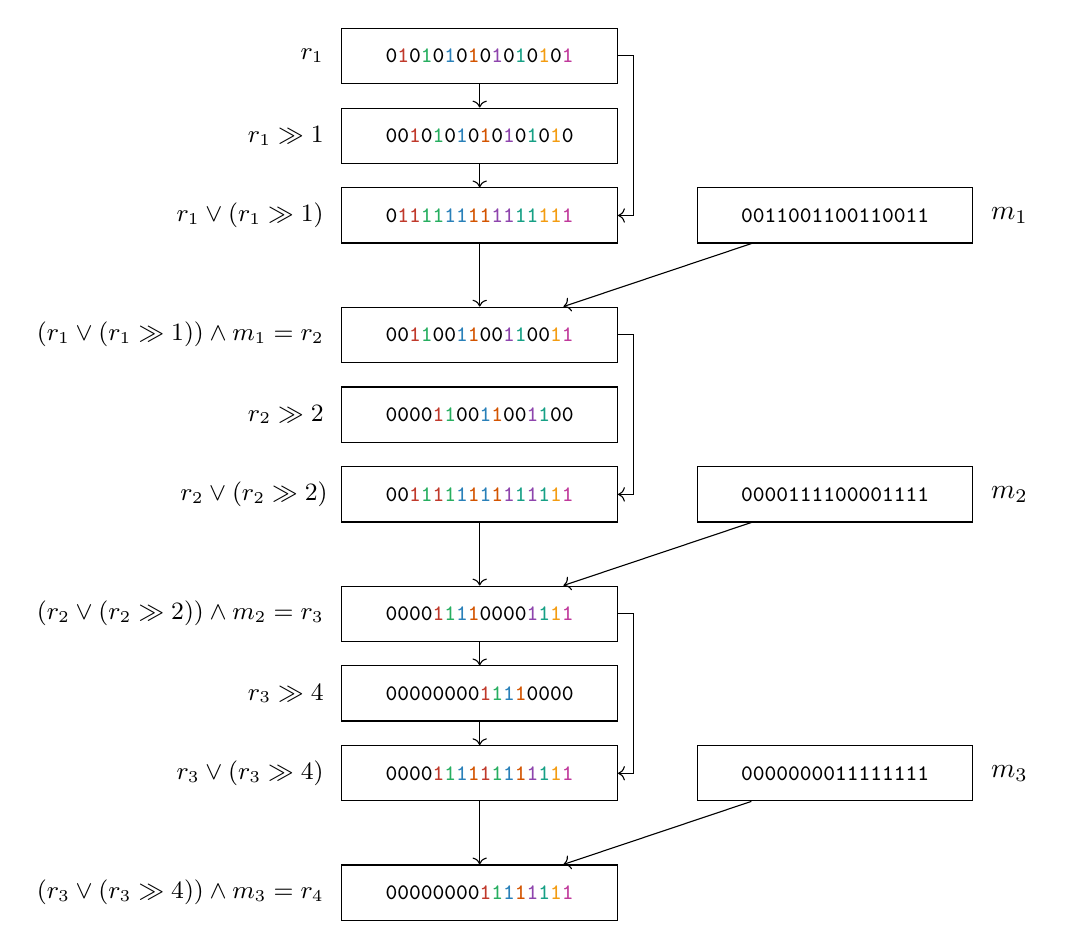
\begin{tikzpicture}[
    node distance=3mm and 3mm, % vertical and horizontal node distance
    bitbox/.style={draw, font=\ttfamily\footnotesize, inner sep=3pt, minimum height=7mm, minimum width=35mm, align=center},
    labelstyle/.style={font=\small, anchor=east},
    oplabelstyle/.style={font=\scriptsize\ttfamily, inner sep=1pt} % For labels like r1, (r1>>1) near |
]

% === Input m ===
% === Stage 1: r1 ===
\node (r1_val)          [bitbox] {\rOnestring};
\node (r1_label)        [labelstyle, left=1mm of r1_val] {$r_1$};

\node (r1_shifted_val)  [bitbox, below=of r1_val] {\rOneshiftedstring};
\node (r1_shifted_label)[labelstyle, left=1mm of r1_shifted_val] {$r_1\gg1$};


\node (v1_val)       [bitbox, below=of r1_shifted_val] {\vOnestring};
\node (s1_R_optext)  [labelstyle, left=1mm of v1_val] {$r_1 \lor (r_1\gg 1)$};

% Operator and Result for Stage 1
\coordinate (s1_op_line_mid_y) at ($(r1_val.east)!0.5!(r1_shifted_val.east)$);
\draw[->] (r1_val) -- (r1_shifted_val);
\draw (r1_val.east) -- ($(r1_val.east)+(2mm,0)$) coordinate (s1_bra_A_right);
\draw[<-] (v1_val.east) -- ($(v1_val.east)+(2mm,0)$) coordinate (s1_bra_B_right);
\draw[->] (r1_shifted_val) -- (v1_val);
\draw (s1_bra_A_right) -- (s1_bra_B_right); % Vertical line of bracket

\node (mask1) [bitbox, right=10mm of v1_val] {0011001100110011};
\node (mask1_label) [right=1mm of mask1] {$m_1$};

% === Stage 2: r2 ===
\node (r2_val)          [bitbox, below=8mm of v1_val] {\rTwostring};
\node (r2_label)        [labelstyle, left=1mm of r2_val] {$(r_1\lor (r_1\gg 1)) \land m_1=r_2$};

\node (r2_shifted_val)  [bitbox, below=of r2_val] {\rTwoshiftedstring};
\node (r2_shifted_label)[labelstyle, left=1mm of r2_shifted_val] {$r_2\gg 2$};

\node (v2_val)       [bitbox, below=of r2_shifted_val] {\vTwostring};
\node (s2_R_optext)  [labelstyle, left=0.5mm of v2_val] {$r_2 \lor (r_2 \gg 2)$};


% Operator and Result for Stage 2
\draw[->] (v1_val) -- (r2_val);
\draw[->] (mask1) -- (r2_val);
\draw (r2_val.east) -- ($(r2_val.east)+(2mm,0)$) coordinate (s2_bra_A_right);
\draw[<-] (v2_val.east) -- ($(v2_val.east)+(2mm,0)$) coordinate (s2_bra_B_right);
\draw (s2_bra_A_right) -- (s2_bra_B_right);

\node (mask2) [bitbox, right=10mm of v2_val] {0000111100001111};
\node (mask2_label) [right=1mm of mask2] {$m_2$};


% === Stage 3: r3 ===
\node (r3_val)          [bitbox, below=8mm of v2_val] {\rThreestring};
\node (r3_label)        [labelstyle, left=1mm of r3_val] {$(r_2 \lor (r_2\gg 2)) \land m_2=r_3$};

\node (r3_shifted_val)  [bitbox, below=of r3_val] {\rThreeshiftedstring};
\node (r3_shifted_label)[labelstyle, left=1mm of r3_shifted_val] {$r_3\gg 4$};

% Operator and Result for Stage 3

\node (v3_val)       [bitbox, below=of r3_shifted_val] {\vThreestring};
\node (s3_L_optext)  [labelstyle, left=1mm of v3_val] {$r_3 \lor (r_3 \gg 4)$};

\draw (r3_val.east) -- ($(r3_val.east)+(2mm,0)$) coordinate (s3_bra_A_right);
\draw[<-] (v3_val.east) -- ($(v3_val.east)+(2mm,0)$) coordinate (s3_bra_B_right);
\draw (s3_bra_A_right) -- (s3_bra_B_right);

\draw[->] (mask2) -- (r3_val);
\draw[->] (v2_val) -- (r3_val);
\draw[->] (r3_val) -- (r3_shifted_val);
\draw[->] (r3_shifted_val) -- (v3_val);

\node (mask3) [bitbox, right=10mm of v3_val] {0000000011111111};
\node (mask3_label) [right=1mm of mask3] {$m_3$};

% === Final Result Display ===
\node (final_result_box) [bitbox, below=8mm of v3_val.south, anchor=north] {\finalResultstring};
\node (final_result_label) [labelstyle, left=1mm of final_result_box] {\((r_3 \lor (r_3\gg 4)) \land m_3=r_4\)};
\draw[->] (v3_val.south) -- (final_result_box.north);
\draw[->] (mask3) -- (final_result_box);

\end{tikzpicture}
\end{document}
